% XCircuit output "salidaB.tex" for LaTeX input from salidaB.eps
\def\putbox#1#2#3#4{\makebox[0in][l]{\makebox[#1][l]{}\raisebox{\baselineskip}[0in][0in]{\raisebox{#2}[0in][0in]{\scalebox{#3}{#4}}}}}
\def\rightbox#1{\makebox[0in][r]{#1}}
\def\centbox#1{\makebox[0in]{#1}}
\def\topbox#1{\raisebox{-0.60\baselineskip}[0in][0in]{#1}}
\def\midbox#1{\raisebox{-0.20\baselineskip}[0in][0in]{#1}}
   \scalebox{1}{
   \normalsize
   \parbox{4.05208in}{
   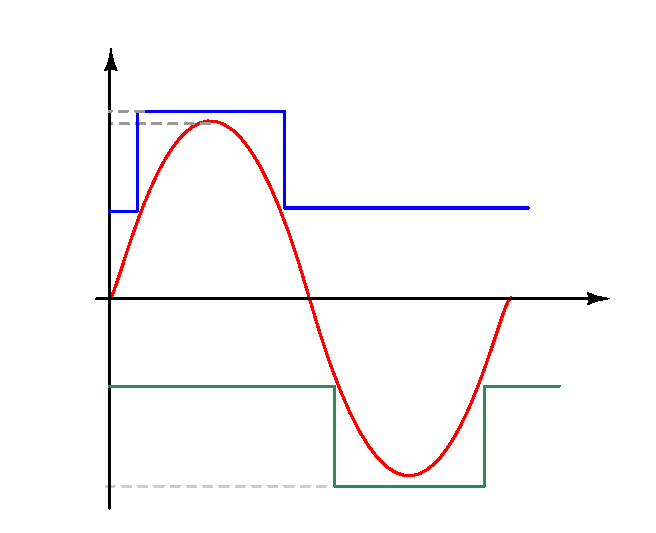
\includegraphics[scale=1]{salidaB}\\
   % translate x=444 y=460 scale 0.38
   \putbox{0.35in}{3.15in}{1.20}{$V_o$}%
   \putbox{4.04in}{1.37in}{1.20}{t}%
   \putbox{0.06in}{2.43in}{1.20}{$\hat{V}_o$}%
   \putbox{3.41in}{1.22in}{1.20}{$T$}%
   \putbox{0.08in}{1.97in}{1.20}{$VccL+$}%
   \putbox{0.20in}{0.81in}{1.20}{$VccL-$}%
   \putbox{0.18in}{0.16in}{1.20}{$VccH-$}%
   \putbox{0.06in}{2.74in}{1.20}{$VccH-$}%
   } % close 'parbox'
   } % close 'scalebox'
   \vspace{-\baselineskip} % this is not necessary, but looks better
